\documentclass[a4paper,12pt]{article}

\usepackage{cmap}
\usepackage{mathtext}
\usepackage[T2A]{fontenc}
\usepackage[utf8]{inputenc}
\usepackage[english,russian]{babel}

\usepackage{amsmath,amsfonts,amssymb,amsthm,mathtools}
\usepackage{icomma}
\usepackage{upgreek}
\mathtoolsset{showonlyrefs=true}

\usepackage{tabto}
\usepackage{euscript}
\usepackage{mathrsfs}

\usepackage{graphicx}

\newcommand*{\hm}[1]{#1\nobreak\discretionary{}
{\hbox{$\mathsurround=0pt #1$}}{}}

\author{Kupriyanov Kirill}
\title{Data Analysis PI\\Theoretical assignment $\#3$}
\date{}

\begin{document}
\maketitle
\thispagestyle{empty}
\newpage
\section*{Task 1.}
\underline{\textit{Problem:}} Consider linear regression task in
one-dimensional space. \({(x_i , y_i)}^N_{i=1}\) is a training dataset and
for object \(i: x_i \in [-1, 1]\) is a feature, $y_i$ is an answer we want to
predict, $y_i^*=kx_i+b$ is our prediction. At the picture below you can see
three different plots of the prediction error \((y - y^*)\) against $x$. Which of
these plots cannot be obtained if least squares method is used to train a
regression model?\\
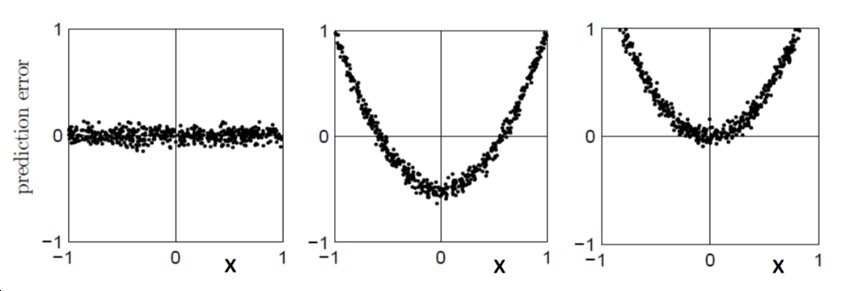
\includegraphics[width=\textwidth]{1}
\newline
\underline{\textit{Solution:}} The first picture represents how data is spread pretty linearly. Obviously, this situation is valid.\\
Pictures 2 and 3 are representing non-linear, but but kind of uniformly
distributed dependencies of features. Also these distributions could roughly be described with the following equation: \(y - \hat{y} = x^2+b\)
\begin{gather}
    y - \hat{y} = x^2 + b\\
    (y - \hat{y})^2 = (x^2 + b^2)^2\\
    \sum^{N}_{i = 1}{(y_i - \hat{y_i})^2} \overset{\text{OLS} }{\rightarrow} \text{min}\\
    \int_{-1}^{1} (y - \hat{y})^2  \rightarrow \text{min}\\
    \text{Now we have } \int_{-1}^{1}(x^2+b)^2\\
    F((x^2+b)^2) = \frac{x^5}{5} + 2b\frac{x^3}{3} + xb^2\\
    \int_{-1}^{1}(x^2 + b)^2 = \frac{1}{5}+\frac{2b}{3} + b^2 + \frac{1}{5} + \frac{2}{3}b + b^2 = \frac{2}{5} + \frac{4}{3}b + 2b^2
\end{gather}
Taking derivative, a value of $b$ could be evaluated. With this $b$, integral reaches its minimum ponts.
\begin{gather}
    4b + \frac{4}{3} = 0\\
    b = -\frac{1}{3}
\end{gather}\\
So we get  ($x^2 - \frac{1}{2}$). Second picture is more likely to be chosen
than the trird one.\\
\newline
So the answer that \textit{third} picture could not be obtained.


\newpage
\section*{Task 2.}
Consider linear regression task in one-dimensional space \(y = kx+b\) and two
datasets: \((x_1^1 , y_1^1 ), \dots, (x^1_n , y_n^1 )\) and
\((x_1^2 , y_1^2), \dots, (x^2_m , y_m^2 )\).
Assume that the least squares method is used to train a regression models in this task.
It turns out, that if we train a regression model on the first dataset we obtain a coefficient \(k_1 > 0\).
Similarly, if we train a regression model on the second dataset we obtain a
coefficient \(k_2 > 0\). Is it true that if we train the regression model on
both datasets together then the obtained coefficient \(k\) will also
be positive?
Additionally answer that question if we know that \(\sum_{i=1}^nx_i^1 = 0 \text{ and  } \sum_{i=1}^mx_i^2 = 0\).\\
\newline
\underline{\textit{Solution:}} First case. Suppose, the green dots are
representing the first dataset. Then, the green line is the solution, which
will be given by a regression. For the second dataset there are red dots and
red line respectively.\\
\newline
Obviously, \(k_1 > 0\) and \(k_2 > 0\). The purpule line is the result of fitting using both datasets. As it could be seen, \(k_{purple} < 0\).\\
\newline
So, the answer to the first question is \textit{no}.
\begin{center}
\includegraphics[width=\textwidth]{fit-dataset}
\end{center}





Implementation from the previous task does
overhead. It recomputes class labels at each new split. What could be done is
presorting features over all relevant samples while keeping the label count. It
will reduce the complexity at each node to \(O(N\cdot \log(N))\). Finding
optimal sum of entropies for 2 new child nodes takes \(O(N)\). Entropy for one
node can be calculated within \(O(1)\).\\
So the total cost for all features is \(O(N\cdot D\cdot \log(N))\). And it finds optimal threshold within \(O(N\cdot \log(N))\).

\section*{Task 3.}
\underline{\textit{Problem:}} Consider multiclass
classification task with \(K\) classes. Objects in this task have \(L\) binary
features.  How many different decision trees of depth \(L\) can be constructed
for this task? Two decision trees are different if there is an object in \(\{0,
1\}\) \(L\) which they classify differently.\\
\newline
\underline{\textit{Solution:}} If only binary features are considered and a
binary classification task, then for a training dataset having $L$ features
there are at most \(2^L\) possible instances. Taking into account that there
are $K$ classes in the dataset, there are \(2^{K^L}\) different ways of labeling
all instances, and each labeling corresponds to a different underlying boolean
function that can be represented as a decision tree.

\end{document}

% EOF
